\documentclass[../main.tex]{subfiles}

\begin{document}
    \subsection{Planowanie testów.}

    \begin{table}[H]
        \begin{center}
            \begin{tabular}{ p{8cm}  p{8cm} }
                \multicolumn{2}{c}{ \textbf{Zalety wczesnego planowania}}\\
                \begin{itemize}
                    \item \textbf{wczesne wykrycie} i możliwość zarządzania \textbf{ryzyk}ami
                    \begin{itemize}
                        \item zmniejszenie prawdopodobieństwa i wpływu ryzyka
                    \end{itemize}
                    \item dokładne \textbf{skoordynowanie} nadchodzących \textbf{działań}
                    \item dostarczenie \textbf{wysokiej jakości planu} prac
                \end{itemize}
                &
                \begin{itemize}
                    \item wczesne wykrycie \textbf{ryzyk projektowych} i problemów trudnych /
                    niemożliwych do wykrycia podczas testowania
                    \begin{itemize}
                        \item błędne założenia, brakujące informacje, brak umiejętności
                    \end{itemize}
                    \item dokładniejsze \textbf{dopasowanie} budżetu, wysiłku, czasu, \textbf{zasobów} – lepsza priorytetyzacja
                    \item identyfikacja kluczowych komponentów
                \end{itemize}\\
            \end{tabular}
        \end{center}
    \end{table}


    \begin{table}[H]
        \begin{center}
            \begin{tabular}{| p{8cm} | p{8cm} |}
                \hline
                \multicolumn{2}{|c|}{\textbf{SZACOWANIE}}\\
                \hline
                \hline
                \multicolumn{2}{|p{16cm}|}{ Szacowanie pozwala na lepszą \textbf{alokację zasobów} i lepszą \textbf{organizację} projektu. Jest podstawą do podjęcia
                decyzji o ograniczeniu zakresu projektu, jeśli estymowany koszt lub czas jest zbyt duży.
                }\\
                \hline
                \hline
                \textbf{Rola szacowania} & \textbf{Cechy dobrej estymacji.}\\
                \hline
                \begin{itemize}
                    \item określenie \textbf{pracochłonności} projektu
                    \begin{itemize}
                        \item potrzebne zasoby
                        \item potrzebny czas
                        \item potrzebny wysiłek
                    \end{itemize}
                    \item określenie \textbf{kosztochłonności} projektu
                    \begin{itemize}
                        \item ile będzie kosztować wykonanie zaplanowanych zadań?
                    \end{itemize}
                \end{itemize}

                &
                \begin{itemize}
                    \item oparta na wiedzy i doświadczeniu ekspertów
                    \item wspierana przez wykonawców szacowanej pracy
                    \item możliwie dokładna w określaniu kosztów, zasobów, zadań i ludzi
                    \item oparta na najbardziej prawdopodobnych kosztach, wysiłku i czasie trwania poszczególnych zadań
                \end{itemize}
                \\
                \hline
                \multicolumn{2}{|p{16cm}|}{Szacowanie jest \textbf{trudne}. Problemy wynikają nie tylko z samej natury problemu, lecz także z tzw. \textbf{przyczyn politycznych}.
                }\\
                \hline
                \hline
                \multicolumn{2}{|c|}{\textbf{Techniki szacowania}}\\
                \hline
                \begin{itemize}
                    \item intuicja, zgadywanie, doświadczenie
                    \item estymacja przez analogię
                    \item struktura podziału prac (Work Breakdown Structure)
                    \item estymacja grupowa
                \end{itemize}
                &
                \begin{itemize}
                    \item dane przemysłowe
                    \item analiza punktów testowych (Test Point Analysis) [za TMap]
                    \item modele matematyczne (parametryczne)
                \end{itemize}\\
                \hline
            \end{tabular}
        \end{center}
    \end{table}

    \begin{table}[H]
        \begin{center}
            \begin{tabular}{| p{8cm} | p{8cm} |}
                \hline
                \multicolumn{2}{|c|}{\textbf{DOKUMENTACJA}}\\
                \hline
                \hline
                \textbf{Cele dokumentowania} &  \textbf{Rodzaje dokumentów}\\
                \hline
                \begin{itemize}
                    \item \textbf{opisanie} obowiązujących w organizacji lub projekcie \textbf{reguł, standardów, celów} do osiągnięcia, stanowiących punkt odniesienia podczas prac projektowych
                    \item pomoc w tworzeniu planów
                    \item potwierdzanie wykonania określonych czynności
                    \item akceptowanie/zezwalanie na wykonanie określonych czynności
                    \item utrwalenie danych
                    \item pomoc w monitorowaniu i kontroli procesów (actual vs. planned)
                    \item pomoc w opanowaniu złożoności projektów
                    \item mniej lub bardziej formalna \textbf{platforma komunikacji}
                \end{itemize}
                &
                \begin{itemize}
                    \item \textbf{Polityka testów} – wysokopoziomowy opis \textbf{zasad, podejść} i głównych \textbf{zadań} organizacji dotyczących testowania.
                    \item \textbf{Strategia testów} – wysokopoziomowy opis \textbf{poziomów} testów do wykonania oraz testów w ramach tych poziomów dla organizacji lub programu.
                    \item \textbf{Plan testów} – opis \textbf{zakresu, metod, zasobów i harmonogramu} czynności testowych dla projektu; określa m.in. elementy, zadania i środowisko testowe, przydział obowiązków, wykorzystane techniki, kryteria wejścia i wyjścia, ryzyka wymagające ciągłego planowania.
                    \item \textbf{Dziennik wykonania testów} – \textbf{zapis czynności} występujących podczas uruchamiania i wykonywania testów.
                \end{itemize}\\
                \hline
            \end{tabular}
        \end{center}
    \end{table}


    \subsubsection{Metryki}

    \textbf{Nadzór i kontrola postępu testów}. Cel: monitorowanie procesu testowego i reagowanie gdy trzeba.

    \begin{table}[H]
        \begin{center}
            \begin{tabular}{p{8cm} p{8cm}}
                \multicolumn{2}{c}{\textbf{ Na podstawie metryk możemy:}}\\
                \begin{itemize}
                    \item \textbf{mierzyć postęp} procesu testowego
                    \item \textbf{obliczyć zwrot} z inwestycji (ROI), tzn. czy proces testowy daje pożądane korzyści
                    \item \textbf{ocenić} i porównać różne możliwe \textbf{podejścia} do testowania
                    \item \textbf{ocenić} i kontrolować \textbf{wydajność} procesu testowego
                \end{itemize}
                &
                \begin{itemize}
                    \item \textbf{ocenić} i kontrolować \textbf{poprawę} procesu testowego
                    \item \textbf{zbudować system „wczesnego ostrzegania”}
                    \item \textbf{zbudować modele predykcyjne}
                    \item porównywać proces z procesami \textbf{konkurencji}
                \end{itemize}\\
            \end{tabular}
        \end{center}
    \end{table}

    \begin{figure}[H]
        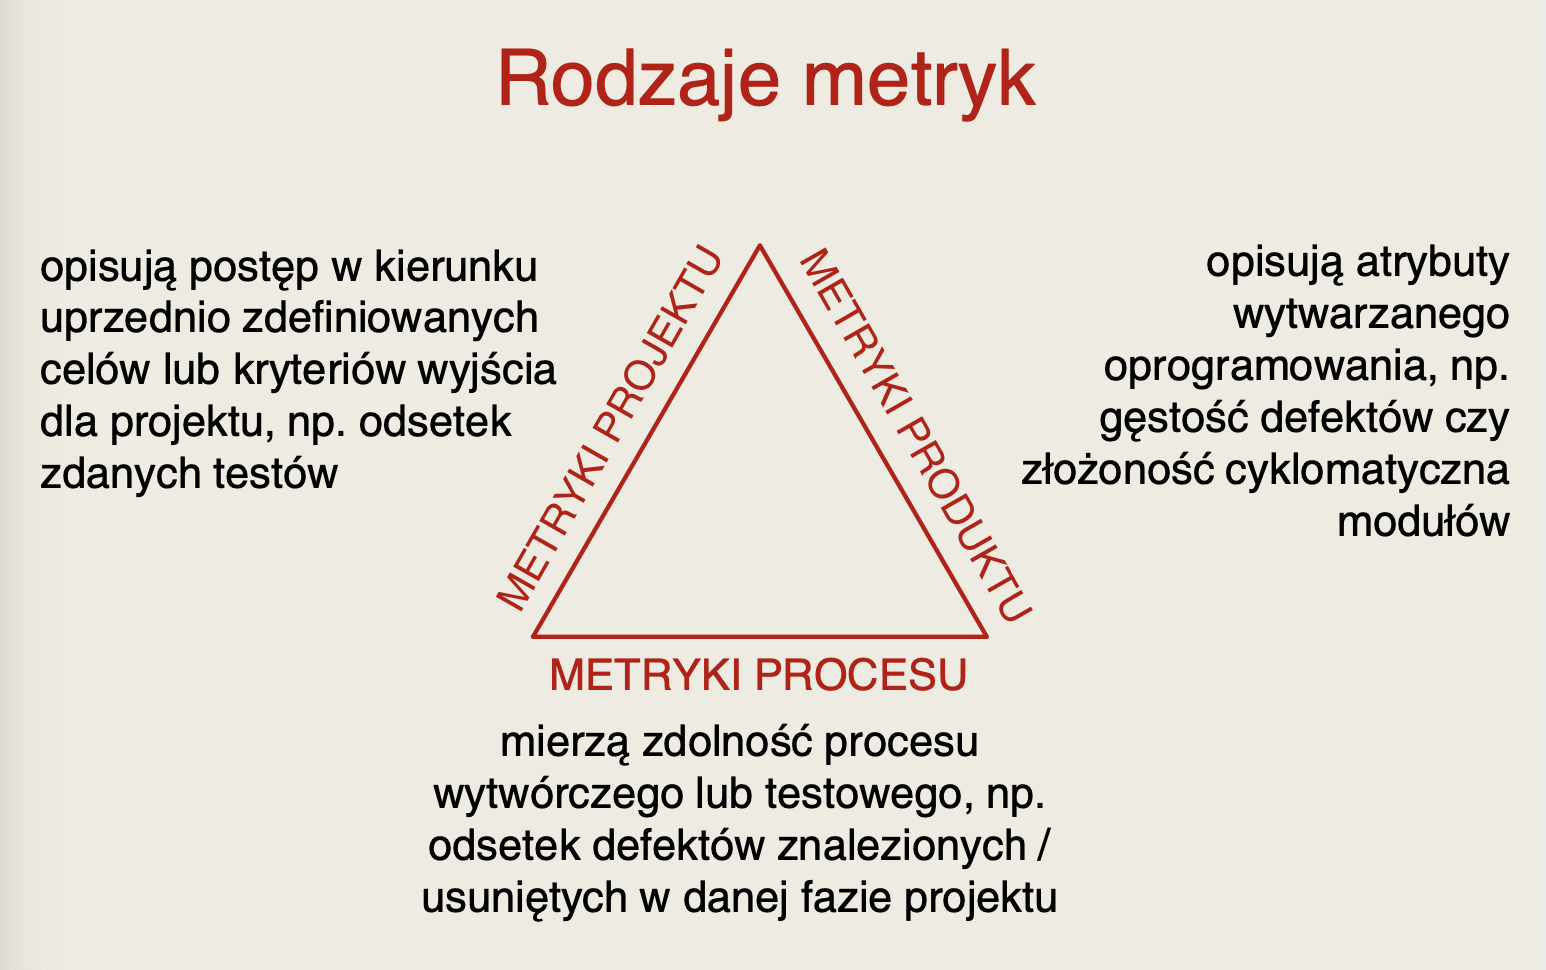
\includegraphics[width=\linewidth]{metryki.png}
    \end{figure}

    \textbf{Wymiary postępu testowania.}
    \begin{itemize}
        \item Ryzyka, defekty, testy i pokrycie – \textbf{metryki ilościowe}
        \item Pewność – najbardziej subiektywna, często \textbf{jakościowa}; pomiar za pomocą ankiet, wywiadów, kwesionariuszy
    \end{itemize}


    \begin{table}[H]
        \begin{center}
            \begin{tabular}{| p{8cm} | p{8cm} |}
                \hline
                \multicolumn{2}{|c|}{\textbf{Przykłady metryk}}\\
                \hline
                \hline
                \textbf{metryki ryzyka produktowego} & \textbf{metryki defektów}\\
                \hline
                \begin{itemize}
                    \item \% ryzyk pokrytych przez zdane testy
                    \item \% ryzyk, dla których co najmniej jeden test nie przeszedł
                    \item \% ryzyk nieprzetestowanych w całości
                    \item \% pokrytych ryzyk podzielonych wg kategorii ryzyka
                    \item \% ryzyk zidentyfikowanych po wstępnej analizie ryzyka
                    \item liczba zidentyfikowanych ryzyk w czasie
                \end{itemize}
                &
                \begin{itemize}
                    \item skumulowana liczba zgłoszonych/naprawionych/otwartych defektów
                    \item średni czas między awariami (MTBF)
                    \item średni czas bezawaryjnej pracy (MTTF)
                    \item liczba/częstotliwość zgłaszania defektów/awarii
                    \item średni czas naprawy
                    \item liczba źle wykonanych napraw
                \end{itemize}\\
                \hline
            \end{tabular}
        \end{center}
    \end{table}

    \begin{table}[H]
        \begin{center}
            \begin{tabular}{| p{8cm} | p{8cm} |}
                \hline
                \textbf{metryki przypadków testowych} & \textbf{metryki pokrycia}\\
                \hline
                \begin{itemize}
                    \item całkowita liczba zaprojektowanych, zaimplementowanych, wykonanych, zdanych, niezdanych, zawieszonych, pominiętych przypadków testowych
                    \item liczba testów w podziale na moduły, poziomy, fazy testowania
                    \item stan testów regresji i testów potwierdzających
                    \item dostępność środowiska testowego
                    \item średni czas wykonywania testu
                \end{itemize}
                &
                \begin{itemize}
                    \item liczba (\%) pokrytych wymagań, elementów projektowych, modułów, konfiguracji, ryzyk
                    \item stopień pokrycia kodu, warunków, rozgałęzień, decyzji itp.
                    \item stopień pokrycia klas równoważności, wartości brzegowych, stanów maszyny stanowych i innych elementów pokrycia dla testów czarnoskrzynkowych
                \end{itemize}\\
                \hline
                \hline
                \textbf{metryki pewności} &\\
                \hline
                powinny uwzględnić przynajmniej następujące zagadnienia
                \begin{itemize}
                    \item stabilność, niezawodność, dostępność systemu
                    \item liczba defektów
                    \item nierozwiązane problemy krytyczne
                    \item wstępna ocena klienta
                    \item inne parametry jakości istotne dla danego produktu, wymagań klienta i rynku
                \end{itemize} &\\
                \hline
            \end{tabular}
        \end{center}
    \end{table}


    \subsection{Zarządzanie incydentami}
    \textbf{Kiedy usterka może być wykryta?}
    \begin{table}[H]
        \begin{center}
            \begin{tabular}{p{8cm} p{8cm}}
                \begin{itemize}
                    \item podczas testowania \textbf{statycznego}
                    \begin{itemize}
                        \item przeglądy wymagań
                        \item przeglądy projektu
                        \item przeglądy kodu
                        \item analiza kodu
                    \end{itemize}
                \end{itemize}
                &
                \begin{itemize}
                    \item podczas testowania\textbf{dynamicznego}
                    \begin{itemize}
                        \item wynik oczekiwany $\neq$ wynik rzeczywisty
                        \item defekt nie musi być w kodzie – może być w teście!
                    \end{itemize}
                \end{itemize}
            \end{tabular}
        \end{center}
    \end{table}

    \subsubsection{IEEE 1044.}
    Cykl życia defektu wg IEEE 1044.
    \begin{enumerate}
        \item \textbf{Rozpoznanie (recognition)} – zaobserwowanie anomalii (incydent) wskazującej na potencjalny defekt – może nastąpić w dowolnej fazie cyklu życia oprogramowania
        \item \textbf{Badanie (investigation)} – badanie incydentu; może wykryć powiązane problemy i zaproponować rozwiązania
        \item \textbf{Działanie (action)} – możemy chcieć rozwiązać defekt lub podjąć akcje zapobiegania wystąpienia podobnych defektów w przyszłości; po rozwiązaniu muszą nastąpić testy regresji i testy potwierdzające; testy dotychczas blokowane przez defekt mogą zostać wykonane
        \item \textbf{Dyspozycja (disposition)} – zbieranie dalszych informacji i przeniesienie defektu w stan końcowy
    \end{enumerate}

    \begin{figure}[H]
        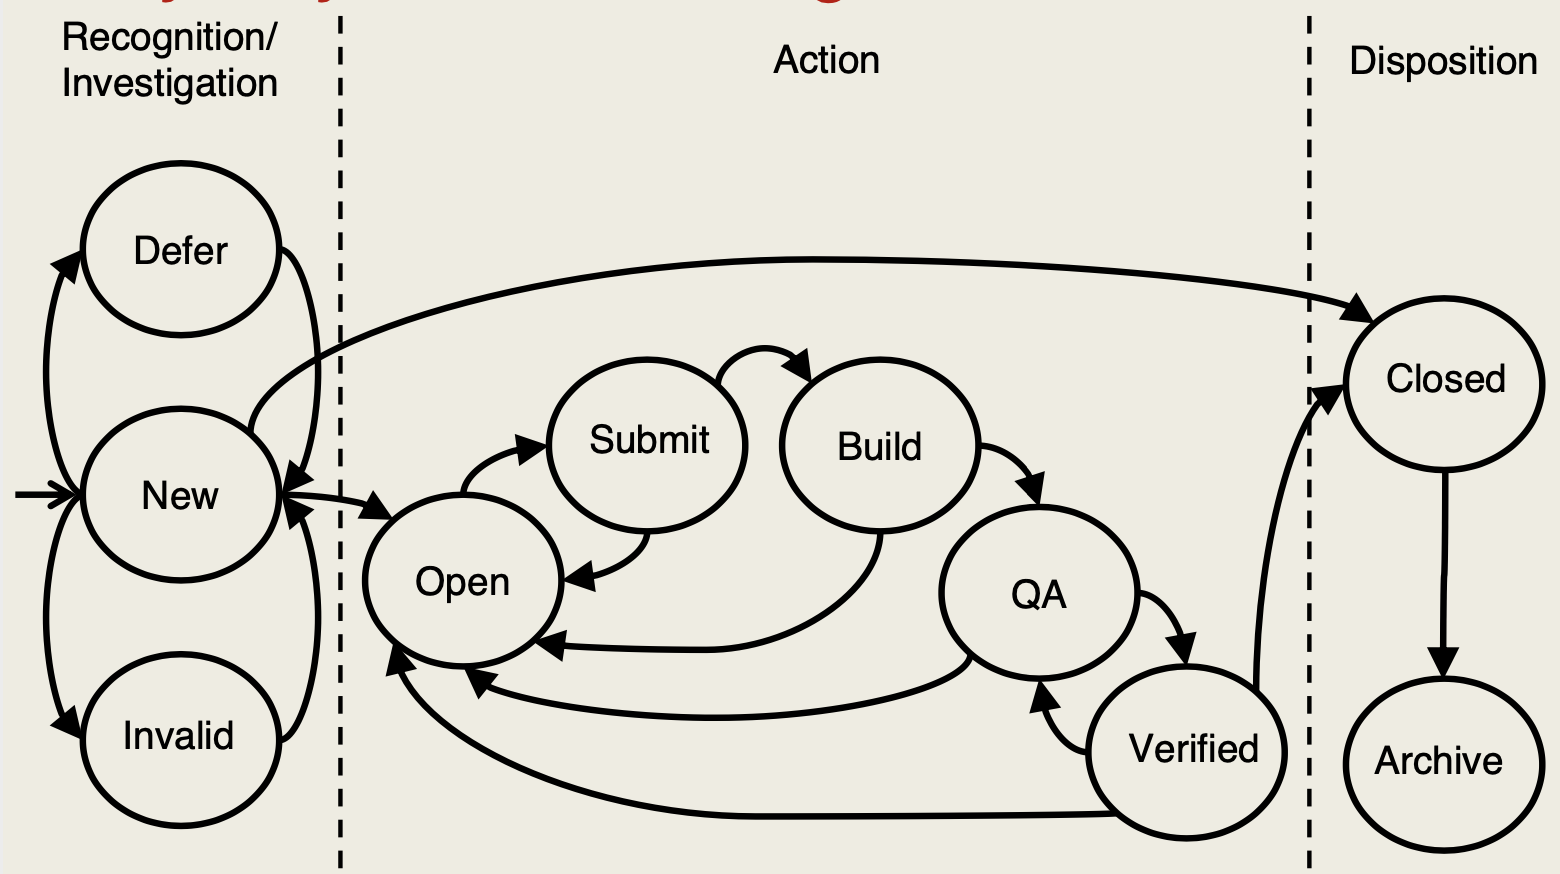
\includegraphics[width=\linewidth]{ieee1044.png}
    \end{figure}


    \begin{table}[H]
        \begin{center}
            \begin{tabular}{ | p{3cm} | p{3cm} | p{3cm} | p{3cm} |}
                \hline
                \multirow{2}{*}{\textbf{Krok}} & \multicolumn{3}{c|}{\textbf{Czynności}}\\
                \cline{2-4}
                \multirow{2}{*}{} & \textbf{rejestruj}\ldots & \textbf{klasyfikuj}\ldots & \textbf{identyfikuj wpływ}\ldots\\
                \hline
                \textbf{Rozpoznanie }& wspomagające informacje
                & na podstawie ważnych atrybutów
                & na podstawie postrzeganego wpływu\\
                \hline
                \textbf{Badanie}
                & zaktualizuj i dodaj dodatkowe informacje
                & zaktualizuj i dodaj klasyfikację na podst. ważnych atrybutów
                & aktualizuj na podstawie badania\\
                \hline
                \textbf{Działanie}
                & dodaj dane oparte o podjęte działanie
                & dodaj dane oparte o podjęte działanie
                & aktualizuj na podstawie działania\\
                \hline
                \textbf{Dyspozycja}
                & dodaj dane bazujące na dyspozycji
                & na podstawie dyspozycji
                & aktualizuj na podstawie dyspozycji\\
                \hline
            \end{tabular}
        \end{center}
    \end{table}


    \begin{table}[H]
        \begin{center}
            \begin{tabular}{| p{8cm} | p{8cm} |}
                \hline
                \textbf{Atrybuty defektu wg IEEE 1044} &   \textbf{Klasyfikacje wpływu defektu wg IEEE 1044}\\
                \hline
                zgłoszenie defektu pozwalające na podjęcie działania jest:
                \begin{itemize}
                    \item \textbf{kompletne} - nie brakuje żadnych ważnych szczegółów,
                    \item \textbf{zwięzłe} - nie zawiera nieistotnych informacji,
                    \item \textbf{precyzyjne} - nie wprowadza czytelnika w błąd,
                    \item \textbf{obiektywne} - bazuje na faktach, nie atakuje nikogo.
                \end{itemize}
                &

                \begin{itemize}
                    \item dotkliwość (severity)
                    \item priorytet
                    \item wartość dla klienta
                    \item sukces misji (mission safety)
                    \item harmonogram projektu
                    \item koszt projektu
                    \item ryzyko projektu
                    \item jakość projektu
                    \item kwestie społeczne
                \end{itemize}\\
                \hline
            \end{tabular}
        \end{center}
    \end{table}

    \subsubsection{Główne modele doskonalenia}
    \begin{table}[H]
        \begin{center}
            \begin{tabular}{p{8cm} p{8cm}}
                \begin{itemize}
                    \item Test Maturity Model (TMM)
                    \item Test Process Improvement (TPI, TPI Next)
                    \item Critical Testing Processes (CTP)
                    \item Systematic Test and Evaluation Process (STEP)
                \end{itemize}
                &
                \begin{itemize}
                    \item Test Organization Maturity (TOM)
                    \item Test Improvement Model (TIM)
                    \item Software Quality Rank (SQR)
                    \item TMap
                \end{itemize}
            \end{tabular}
        \end{center}
    \end{table}


    \begin{figure}[H]
        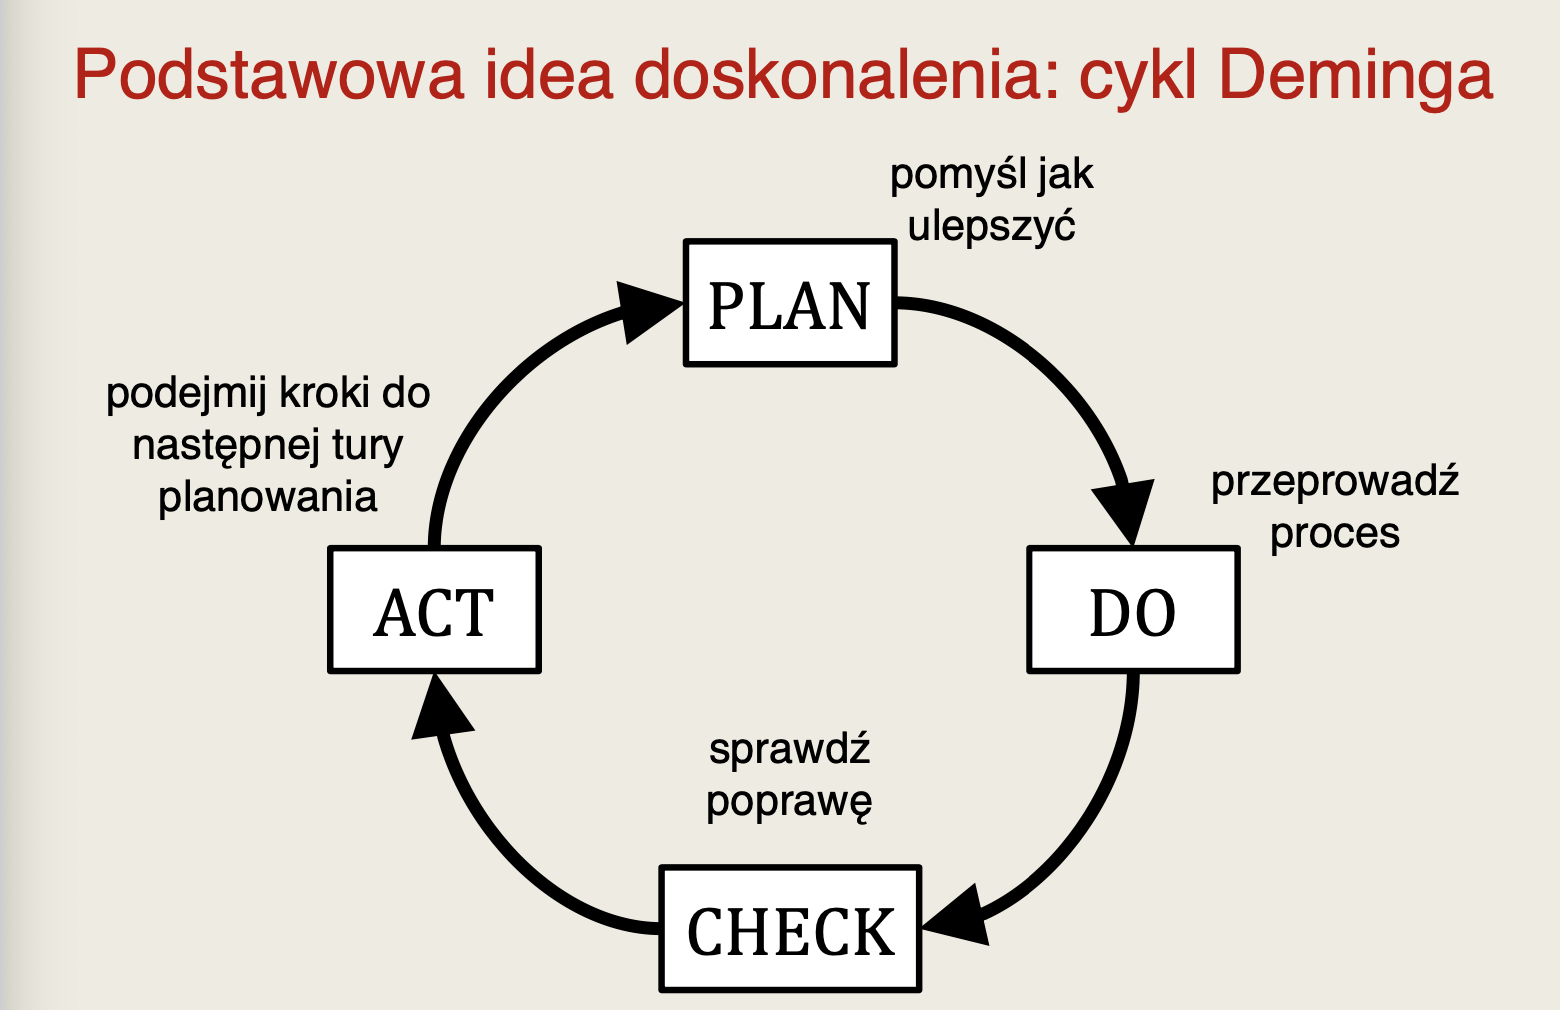
\includegraphics[width=\linewidth]{deming.png}
    \end{figure}

    \begin{table}[H]
        \begin{center}
            \begin{tabular}{| p{8cm} | p{8cm} |}
                \hline
                \multicolumn{2}{|c|}{\textbf{Modele referencyjne}}\\
                \textbf{procesu} & \textbf{zawartości}\\
                \hline
                \begin{itemize}
                    \item (jednowymiarowa) ocena dojrzałości procesu
                    \item wskazują kolejność usprawnień
                \end{itemize}
                &
                \begin{itemize}
                    \item opisują ważne procesy software’owe i co powinno się z nimi robić
                    \item ale nie szeregują zadań w żadnej kolejności
                \end{itemize}\\
                \hline
            \end{tabular}
        \end{center}
    \end{table}
\end{document}